% This Source Code Form is subject to the terms of the Mozilla Public
% License, v. 2.0. If a copy of the MPL was not distributed with this
% file, You can obtain one at https://mozilla.org/MPL/2.0/.

\documentclass[a4paper, 12pt]{article}

\usepackage[english, russian]{babel}
\usepackage[T2A]{fontenc}
\usepackage[utf8]{inputenc}
\setlength{\parindent}{1cm}
\usepackage{graphicx}
\usepackage{amsmath}
\usepackage{amssymb}
\usepackage{amsfonts}
\usepackage{array}
\usepackage{booktabs}
\usepackage{wrapfig}
\usepackage{caption} %заголовки плавающих объектов
\captionsetup[table]{justification=centering} %установки для заголовков таблиц
\captionsetup[figure]{justification=centering} %установки для заголовков таблиц

\begin{document}
	\begin{center}
		\subsubsection*{Расчётное задание по математической физике}
		\subsubsection*{Глава №1: Введение}
		\subsubsection*{Выполнил студент третьего курса Физико-механического института, высшей школы ФФИ: Куликовских Илья}
		\subsubsection*{Группа: 5030302/30801}
		\subsubsection*{Вариант 6}
		\subsubsection*{Преподаватель: Елатонцев Вадим Александрович}
	\end{center}
	
	\quad \textbf{Задание 1.01.01} Найти площадь $S$ заключённую между двумя кривыми $f(x) = 2- x^2$; $g(x) = x^2$.
	
	\quad \textbf{Решение. } Построим графики кривых и определим границы области, ограниченной этими кривыми. 
	
	\begin{figure}[htpb]
		\centering 
		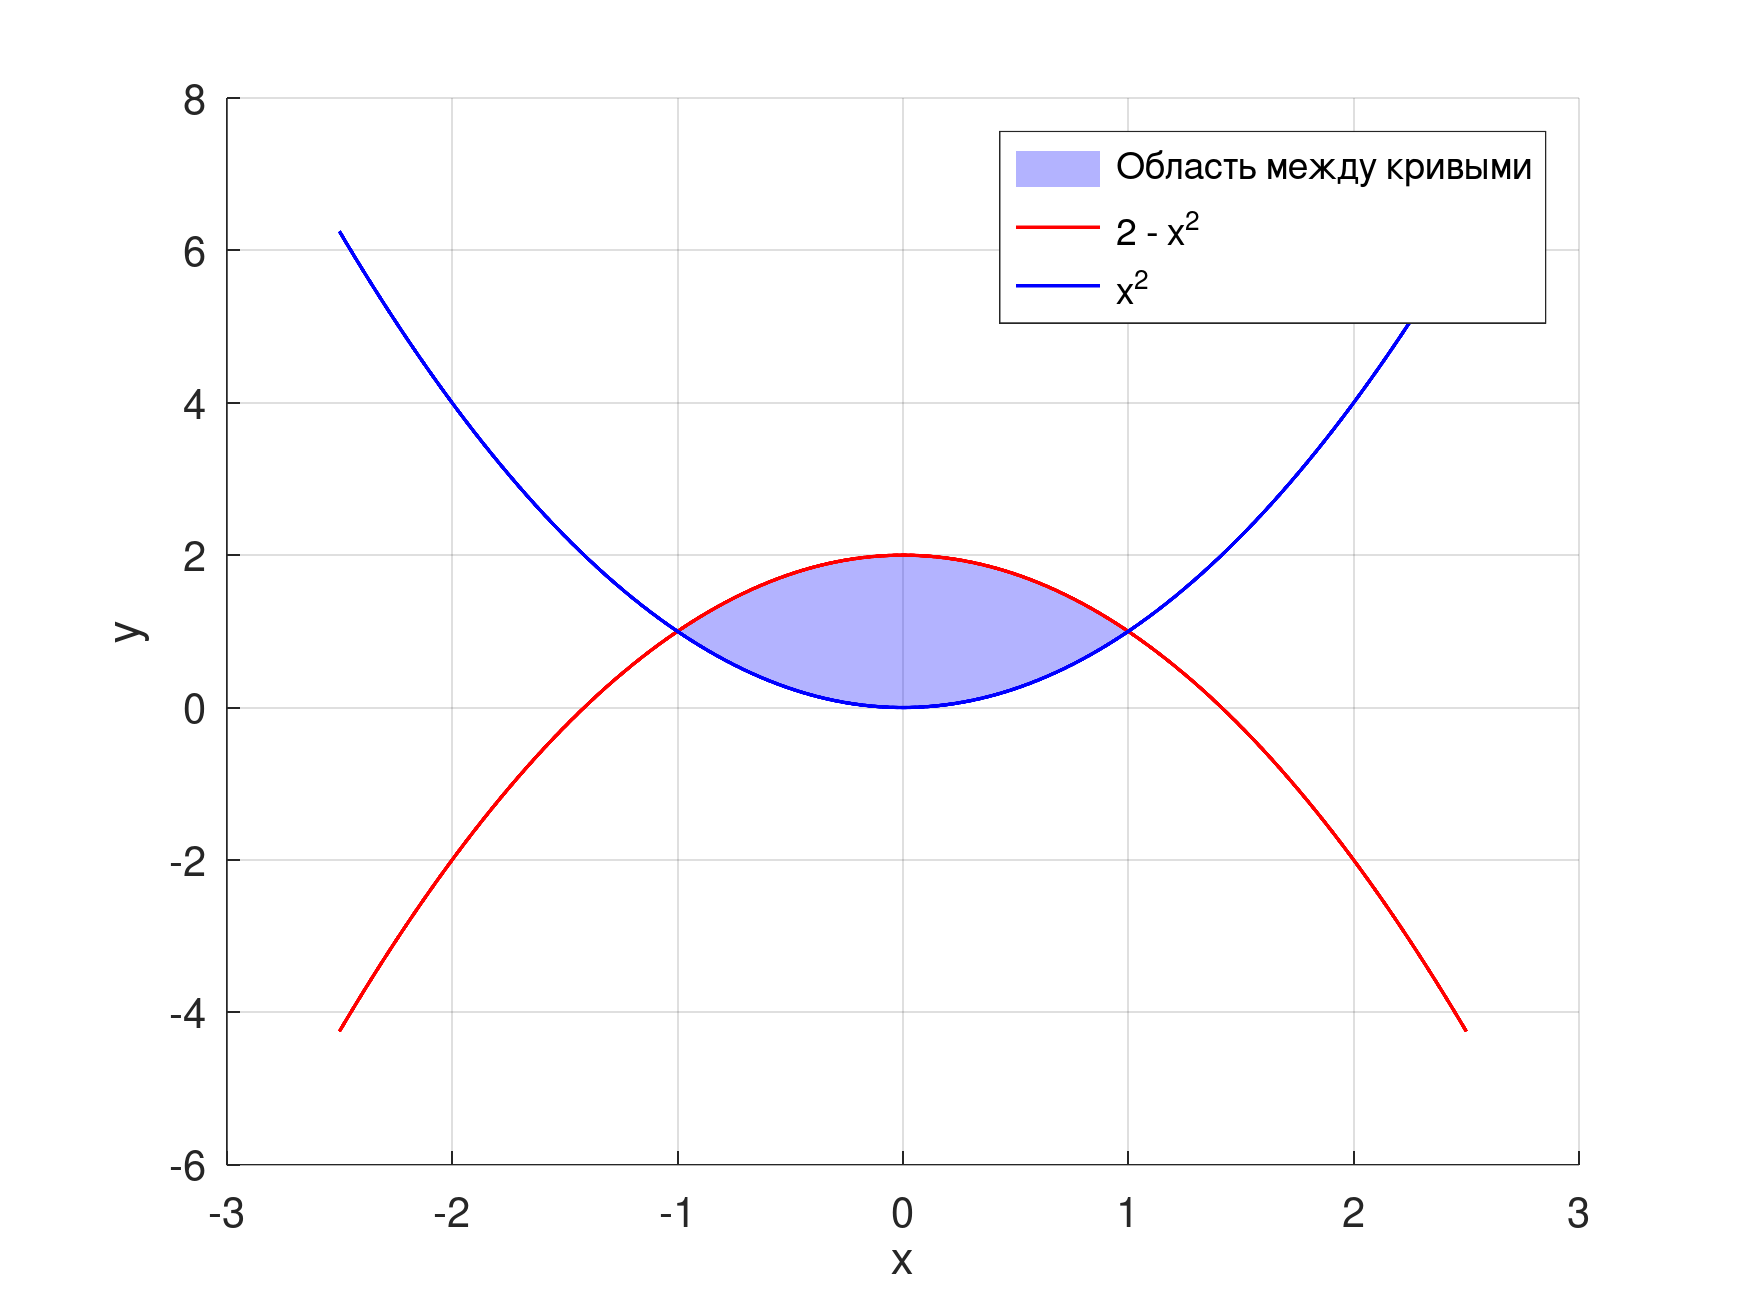
\includegraphics[width=0.8\textwidth]{10101.png}
		\caption{Область между кривыми}
	\end{figure}
	
	\quad Рассмотрим разность интеграллов: 
	
	\begin{center}
		$\displaystyle\int\limits_{-1}^{1} (2 - x^2)dx - \displaystyle\int\limits_{-1}^{1} x^2 dx = 2x\bigg|_{-1}^{1} - \dfrac{2}{3}x^3\bigg|_{-1}^{1}  = \dfrac{8}{3} = S$ 
	\end{center}
	
	\quad \textbf{Ответ:} $S = \dfrac{8}{3}$
	
	\quad \textbf{Задание 1.01.46}  Используя выражение для $\vec{\nabla \psi}$ в декартовой системе  координат, и, используя формулы перехода  от декартовых ортов  $\left(e_x, e_y, e_z\right)$  к ортам сферической системы координат $\left(e_r, e_{\alpha}, e_{\theta}\right)$, а также формулы перехода от декартовых компонент вектора к сферической системе $(x, y, z) \rightarrow (r, \alpha, \theta)$, получить формулу для $\vec{\nabla \psi}$ в  сферической  системе  координат. 
	

	\quad \textbf{Решение.} Распишем выражение для $\vec{\nabla\psi}$ :
	
	\begin{equation}
		\vec{\nabla \psi} = \dfrac{\partial\psi}{\partial x} \vec{e_x} + \dfrac{\partial \psi}{\partial y} \vec{e_y} + \dfrac{\partial \psi}{\partial z} \vec{e_z} 
	\end{equation}
	
	\quad Воспользуемся соотношениями между координатами декартовой и сферической системами отcчёта: 
	
	\begin{equation}
		\begin{cases}
			x = r\sin\theta\cos\alpha  \\
			y = r\sin\theta\sin\alpha  \\
			z = r\cos\theta
		\end{cases}
	\end{equation}
	
	\quad На основе этого составим систему уравнений: 
	
	\begin{equation}
		\begin{cases}
			\dfrac{\partial \psi}{\partial r} = \dfrac{\partial \psi}{\partial x} \dfrac{\partial x}{\partial r} + \dfrac{\partial \psi}{\partial y} \dfrac{\partial y}{\partial r} + \dfrac{\partial \psi}{\partial z}\dfrac{\partial z}{\partial r}\\
			\\
			\dfrac{\partial \psi}{\partial \theta} = \dfrac{\partial \psi}{\partial x} \dfrac{\partial x}{\partial \theta} + \dfrac{\partial\psi}{\partial y} \dfrac{\partial y}{\partial \theta} + \dfrac{\partial \psi}{\partial z} \dfrac{\partial z}{\partial \theta}\\
			\\
			\dfrac{\partial \psi}{\partial \alpha} = \dfrac{\partial \psi}{\partial x} \dfrac{\partial x}{\partial \alpha} + \dfrac{\partial\psi}{\partial y} \dfrac{\partial y}{\partial \alpha} + \dfrac{\partial \psi}{\partial z} \dfrac{\partial z}{\partial \alpha}
		\end{cases} \implies \left[ \begin{array} {ccc|c}
		\dfrac{\partial x}{\partial r} & \dfrac{\partial y}{\partial r} & \dfrac{\partial z}{\partial r} & \dfrac{\partial \psi}{\partial r} \\
		& & & \\
		\dfrac{\partial x}{\partial \theta} & \dfrac{\partial y}{\partial \theta} & \dfrac{\partial z}{\partial \theta} & \dfrac{\partial\psi}{\partial\theta} \\
		& & & \\
		 \dfrac{\partial x}{\partial \alpha} & \dfrac{\partial y}{\partial \alpha} & \dfrac{\partial z}{\partial \alpha} & \dfrac{\partial\psi}{\partial\alpha} \\
		\end{array} \right] \implies 
	\end{equation}
	
	
		$\implies \Delta = \dfrac{\partial x}{\partial r} \left( \dfrac{\partial y}{\partial \theta}\dfrac{\partial z}{\partial \alpha} - \dfrac{\partial y}{\partial\alpha} \dfrac{\partial z}{\partial\theta}\right) - \dfrac{\partial y}{\partial r} \left( \dfrac{\partial x}{\partial \theta} \dfrac{\partial z}{\partial \alpha } - \dfrac{\partial x }{\partial \alpha} \dfrac{\partial z}{\partial \theta }\right) + \newline +\dfrac{\partial z}{\partial r} \left( \dfrac{\partial x}{\partial \theta} \dfrac{\partial y}{\partial \alpha} - \dfrac{\partial x}{\partial \alpha}\dfrac{\partial y}{\partial \theta} \right) = r^2\sin^3\theta\cos^2\alpha + r^2 \sin^3\theta\sin^2\alpha +  r^2\cos^2\theta\cos^2\alpha\sin\theta  + + r^2\cos^2\theta\sin^2\alpha\sin\theta = r^2 \sin\theta \newline$ 
		
		$\Delta_x =  \dfrac{\partial \psi}{\partial r} \left( \dfrac{\partial y}{\partial \theta}\dfrac{\partial z}{\partial \alpha} - \dfrac{\partial y}{\partial\alpha} \dfrac{\partial z}{\partial\theta}\right) - \dfrac{\partial y}{\partial r} \left( \dfrac{\partial \psi}{\partial \theta} \dfrac{\partial z}{\partial \alpha } - \dfrac{\partial \psi }{\partial \alpha} \dfrac{\partial z}{\partial \theta }\right) + \newline + \dfrac{\partial z}{\partial r} \left( \dfrac{\partial \psi}{\partial \theta} \dfrac{\partial y}{\partial \alpha} - \dfrac{\partial \psi}{\partial \alpha}\dfrac{\partial y}{\partial \theta} \right) = r^2\sin^2\cos\alpha\dfrac{\partial\psi}{\partial r} - \dfrac{\partial \psi}{\partial \alpha} r\sin^2\theta\sin\alpha + \dfrac{\partial\psi}{\partial\theta}r\sin\theta\cos\theta\cos\alpha - - \dfrac{\partial\psi}{\partial\alpha}r\cos^2\theta\sin\alpha = \dfrac{\partial \psi}{\partial r}r^2\sin^2\theta \cos\alpha + \dfrac{\partial\psi}{\partial\theta}r\sin\theta\cos\theta\cos\alpha - \dfrac{\partial\psi}{\partial\alpha}r\sin\alpha$
		
		$\Delta_y =  \dfrac{\partial x}{\partial r} \left( \dfrac{\partial \psi}{\partial \theta}\dfrac{\partial z}{\partial \alpha} - \dfrac{\partial \psi}{\partial\alpha} \dfrac{\partial z}{\partial\theta}\right) - \dfrac{\partial \psi}{\partial r} \left( \dfrac{\partial x}{\partial \theta} \dfrac{\partial z}{\partial \alpha } - \dfrac{\partial x }{\partial \alpha} \dfrac{\partial z}{\partial \theta }\right) + \newline \dfrac{\partial z}{\partial r} \left( \dfrac{\partial x}{\partial \theta} \dfrac{\partial \psi}{\partial \alpha} - \dfrac{\partial x}{\partial \alpha}\dfrac{\partial \psi}{\partial \theta} \right) = \dfrac{\partial \psi}{\partial \alpha}r\sin^2\theta\cos\alpha + \dfrac{\partial\psi}{\partial r}r^2 \sin^2\theta \sin\alpha + \dfrac{\partial \psi}{\partial \alpha} r \cos^2\theta\cos\alpha + \dfrac{\partial \psi}{\partial \theta} r\sin\theta\sin\alpha\cos\theta = \dfrac{\partial \psi}{\partial\alpha} r\cos\alpha + \dfrac{\partial\psi}{\partial r}r^2 \sin^2\theta \sin\alpha + \dfrac{\partial \psi}{\partial \theta} r\sin\theta\sin\alpha\cos\theta$
		
		$\Delta_z =  \dfrac{\partial x}{\partial r} \left( \dfrac{\partial y}{\partial \theta}\dfrac{\partial \psi}{\partial \alpha} - \dfrac{\partial y}{\partial\alpha} \dfrac{\partial \psi}{\partial\theta}\right) - \dfrac{\partial y}{\partial r} \left( \dfrac{\partial x}{\partial \theta} \dfrac{\partial \psi}{\partial \alpha } - \dfrac{\partial x }{\partial \alpha} \dfrac{\partial \psi}{\partial \theta }\right) + \newline \dfrac{\partial \psi}{\partial r} \left( \dfrac{\partial x}{\partial \theta} \dfrac{\partial y}{\partial \alpha} - \dfrac{\partial x}{\partial \alpha}\dfrac{\partial y}{\partial \theta} \right) = \dfrac{\partial\psi}{\partial\alpha}r\cos\theta\sin\theta\cos\alpha\sin\alpha - \dfrac{\partial\psi}{\partial\theta}r\sin^2\theta\cos\alpha - \dfrac{\partial\psi}{\partial\alpha}r\sin\theta\cos\theta\cdot \newline \cdot \sin\alpha\cos\alpha - \dfrac{\partial\psi}{\partial\theta}r\sin^2\theta\sin^2\alpha +\dfrac{\partial\psi}{\partial\psi}r\cos\theta\cos^2\alpha\sin\theta + \dfrac{\partial\psi}{\partial r}r\sin\theta\cos\theta\sin^2\alpha = -\dfrac{\partial \psi}{\partial\theta} r\sin^2\theta + \dfrac{\partial\psi}{\partial r} r^2\sin\theta\cos\theta$

	
	\begin{equation}
		\dfrac{\partial \psi}{\partial x} = \dfrac{\Delta_x}{\Delta} = \dfrac{\partial \psi}{\partial r} \sin\theta\cos\alpha + \dfrac{1}{r}\dfrac{\partial\psi}{\partial\theta}\cos\theta\cos\alpha - \dfrac{1}{r\sin\theta}\dfrac{\partial\psi}{\partial\alpha}\sin\alpha 		
	\end{equation}
	
	\begin{equation}
		\dfrac{\partial \psi}{\partial y} = \dfrac{\Delta_y}{\Delta} = \dfrac{\cos\alpha}{r\sin\theta}\dfrac{\partial\psi}{\partial\alpha} + \dfrac{\partial\psi}{\partial r}\sin\theta\sin\alpha + \dfrac{1}{r}\dfrac{\partial \psi}{\partial\theta}\sin\alpha\cos\alpha 
	\end{equation}
	
	\begin{equation}
		\dfrac{\partial \psi}{\partial z} = \dfrac{\Delta_z}{\Delta}= \cos\theta \dfrac{\partial \psi}{\partial r} - \dfrac{\sin\theta}{r} \dfrac{\partial \psi}{\partial \theta}
	\end{equation}
		
	\quad Используя соотношения (4)-(6) перепишем заново формулу (1):
	
	
		$\vec{\nabla \psi} = \dfrac{\partial\psi}{\partial x}\vec{e_x} + \dfrac{\partial \psi}{\partial y}\vec{e_y} + \dfrac{\partial \psi}{\partial z}\vec{e_z} = \dfrac{\partial \psi}{\partial r} \left( \sin\theta\cos\alpha\vec{e_x} + \sin\theta\sin\alpha\vec{e_y} + \cos\theta\vec{e_z}\right) + +\dfrac{1}{r}\dfrac{\partial\psi}{\partial\theta} \left( \cos\alpha\cos\theta\vec{e_x} + \sin\alpha\cos\theta\vec{e_y} -\sin\theta\vec{e_z} \right) + \dfrac{1}{r\sin\theta}\dfrac{\partial\psi}{\partial\alpha} \left(-\sin\alpha\vec{e_x} + \cos\alpha\vec{e_y}\right) $
	
	\begin{equation}
		\vec{\nabla \psi} = \dfrac{\partial\psi}{\partial r}\vec{e_r} + \dfrac{1}{r}\dfrac{\partial\psi}{\partial\theta}\vec{e_\theta} + \dfrac{1}{r\sin\theta}\dfrac{\partial\psi}{\partial\alpha}\vec{e_\alpha} \text{ } \blacksquare.
	\end{equation}
	
	\begin{equation}
		\text{Где: } \begin{cases}
			\vec{e_r} = \sin\theta\cos\alpha \vec{e_x} + \sin\theta\sin\alpha\vec{e_y} + \cos\theta\vec{k} \\
			\vec{e_\theta} = \cos\alpha\cos\theta\vec{e_x} + \sin\alpha\cos\theta\vec{e_y} -\sin\theta\vec{e_z} \\
			\vec{e_\alpha} =  -\sin\alpha\vec{e_x} + \cos\alpha\vec{e_y} \\
		\end{cases} 
	\end{equation}
		
	\quad \textbf{Задание 1.01.53} Доказать соотношение:
	\newline
	\begin{center}
		$\displaystyle\iint\limits_{\partial V} \left(\vec{n} \cdot \vec{b} \right) A(\vec{r}) dS = \displaystyle\iiint\limits_{V} \left(\vec{b} \cdot \vec{\nabla} \right) A(\vec{r}) dV$
	\end{center}
	
	\quad где $\vec{n}$ -единичный орт поверхности,  $V$ - объем  пространства с поверхностью, $\vec{b}$ - постоянный  вектор, $A(\vec{r}): \mathbb{R}^3 \rightarrow \mathbb{R} $ скалярное поле.
	
	\quad \textbf{Решение. } Рассмотрим левую часть равенства отдельно: 
	
	\begin{equation}
		\displaystyle\iint\limits_{\partial V} \left(\vec{b}\cdot \vec{n}\right) A(r) dS = \displaystyle\iint\limits_{\partial V} A(r)\vec{b} \cdot \vec{dS} = \displaystyle\iiint\limits_{V} div\left(A(r) \vec{b}\right) dV
	\end{equation}
	
	\quad Отдельно рассмотрим дивергенцию под ингралом: 
	
	\begin{equation}
		div\left(A(r)\vec{b}\right) = \vec{b}\cdot \vec{grad A(r)} + \underbrace{A(r)div( \vec{b})}_{=0} =  \vec{b}\cdot \vec{\nabla} A(r)
	\end{equation}
	
	\begin{equation}
		\displaystyle\iiint\limits_{V} div\left(A(r) \vec{b}\right) dV = \displaystyle\iiint\limits_{V} \vec{b}\cdot \vec{\nabla }A(r) dV \equiv \displaystyle\iint\limits_{\partial V} \left(\vec{b}\cdot \vec{n}\right) A(r) dS \text{ } \blacksquare.
	\end{equation}
\end{document}